\documentclass{article}
\usepackage{jfrExamplee}
\usepackage{graphicx}
\usepackage{apalike}
\usepackage{setspace}
\usepackage{bibentry}
\usepackage{tablefootnote}
\usepackage{hyperref}
\usepackage[para,online,flushleft]{threeparttable}
\usepackage{amsmath}
\usepackage{xcolor}

%% Uncomment line below for double spacing
%\doublespacing

%this template built off template for NIPS 2004

\title{A Single Wheel Test Rig for Ocean World Rovers}

\author{
Athul Pradeepkumar Girija\thanks{ Use footnote for providing further information
about author (webpage, alternative address). Acknowledgments to
funding agencies should go in the \textbf{Acknowledgments} section
at the end of the paper.} \\
School of Aeronautics and Astronautics\\
Purdue University\\
West Lafayette, IN 47907 \\
\texttt{apradee@purdue.edu} \\
\And
Ye Lu \\
School of Aeronautics and Astronautics \\
Purdue University \\
West Lafayette, IN 47907 \\
\texttt{yelu@purdue.edu} \\
\And
Archit Arora \\
School of Aeronautics and Astronautics \\
Purdue University \\
West Lafayette, IN 47907 \\
\texttt{arora31@purdue.edu} \\
\And
Rachana Agrawal \\
School of Aeronautics and Astronautics \\
Purdue University \\
West Lafayette, IN 47907 \\
\texttt{agrawa77@purdue.edu} \\
\And
Maxim de Jong \\
Thin Red Line Aerospace \\
Chilliwack, British Columbia\\ V2R 5M3, Canada\\
\texttt{maxim@thin-red-line.com} \\
\And
Matt Kent \\
Materials Science and Engineering\\
Smithers \\
Ravenna, Ohio 44266\\
\texttt{mkent@smithers.com} \\
\And
Sarag J. Saikia \\
School of Aeronautics and Astronautics \\
Purdue University \\
West Lafayette, IN 47907 \\
\texttt{ssaikia@purdue.edu} \\
\And
James M. Longuski \\
School of Aeronautics and Astronautics \\
Purdue University \\
West Lafayette, IN 47907 \\
\texttt{longuski@purdue.edu} \\
}

% The \author macro works with any number of authors. There are two commands
% used to separate the names and addresses of multiple authors: \And and \AND.
%
% Using \And between authors leaves it to \LaTeX{} to determine where to break
% the lines. Using \AND forces a linebreak at that point. So, if \LaTeX{}
% puts 3 of 4 authors names on the first line, and the last on the second
% line, try using \AND instead of \And before the third author name.

\begin{document}

\maketitle

\begin{abstract}
Sed ut perspiciatis unde omnis iste natus error sit voluptatem accusantium doloremque laudantium, totam rem aperiam, eaque ipsa quae ab illo inventore veritatis et quasi architecto beatae vitae dicta sunt explicabo. Nemo enim ipsam voluptatem quia voluptas sit aspernatur aut odit aut fugit, sed quia consequuntur magni dolores eos qui ratione voluptatem sequi nesciunt. Neque porro quisquam est, qui dolorem ipsum quia dolor sit amet, consectetur, adipisci velit, sed quia non numquam eius modi tempora incidunt ut labore et dolore magnam aliquam quaerat voluptatem. Ut enim ad minima veniam, quis nostrum exercitationem ullam corporis suscipit laboriosam, nisi ut aliquid ex ea commodi consequatur? Quis autem vel eum iure reprehenderit qui in ea voluptate velit esse quam nihil molestiae consequatur, vel illum qui dolorem eum fugiat quo voluptas nulla pariatur? At vero eos et accusamus et iusto odio dignissimos ducimus qui blanditiis praesentium voluptatum deleniti atque corrupti quos dolores et quas molestias excepturi sint occaecati cupiditate non provident, similique sunt in culpa qui officia deserunt mollitia animi, id est laborum et dolorum fuga. Et harum quidem rerum facilis est et expedita distinctio. Nam libero tempore, cum soluta nobis est eligendi optio cumque nihil impedit quo minus id quod maximes.
\end{abstract}

\section{Introduction}
\label{sec:introduction}
Mobility systems have proven to be of immense value in in-situ planetary exploration over the last five decades since Lunokhod-1, the first successful rover to operate on the lunar surface in 1970 \cite{sanguino201750,kassel1971lunokhod}. As opposed to orbital platforms which can only perform remote-sensing investigations and static landers which provide in-situ data but only for a single site, mobility systems enable in-situ measurements across a range of scientifically interesting sites. A wide range of mobility systems which include rovers, articulated robots, hoppers, helicopters, multicopters, balloons, airplanes, floating platforms, ice drills, and submersibles have been proposed for planetary exploration across the Solar System \cite{iagnemma2004mobile,preumont1997conceptual,fiorini1999hopping,balaram2018mars,hassanalian2018evolution,yajima2009scientific,landis2005venus,mitri2014exploration,weiss2008study,lorenz2018exploring}. 

At the time of writing, NASA's Curiosity rover is operational on the Martian surface since 2012 and the Perseverance rover is scheduled to arrive at Mars in 2021 \cite{welch2013systems,williford2018nasa}. The European Space Agency's Rosalind Franklin rover is scheduled to arrive at Mars in 2022 \cite{vago2017habitability}. The Chinese National Space Agency's Yutu 2 rover is operational on the lunar far side and has become the longest operational lunar rover, breaking Lunokhod-1's previous record of 10.5 months \cite{ling2019close}.

The continued interest and commitment in surface mobility systems despite their inherently higher costs compared to orbiter and lander missions underscore their importance in future planetary exploration. However, the poorly known surface properties and features (loose sand, large boulders, sharp rocks etc.) present significant engineering challenges to surface mobility systems. Perhaps the most notable example is NASA's Spirit rover became trapped in soft sand and could not gain traction to free itself, eventually leading to a loss of mission \cite{lorenz2014moving}. Prior to the embedding event, the Spirit rover had experienced significant slippage when crossing fine-grained surfaces \cite{li2008characterization}. The twin rover Opportunity has also been subject to such near-embedding events as it traversed deformable sand terrain \cite{zhou2014simulations,arvidson2011opportunity}. Similar slippage and sinkage problems were encountered by the Curiosity rover when crossing ripple fields \cite{arvidson2014roving}; in addition to significant wheel damage from traversing over sharp rock outcrops \cite{arvidson2017relating}. These experiences make it clear that a thorough understanding of the wheel-soil/terrain interaction is of critical importance for planning future missions which include surface mobility systems. The Mars rovers used a combination of numerical modeling, single-wheel test rig experiments, and full vehicle field tests in analog sites such as the Mojave Desert to characterize the wheel-terrain interaction and predict vehicle performance. Based on the data, the mission operations team selects the best possible path so as to minimize the risk of undesirable events such as embedding in a sand trap.

While the majority of the existing literature in the field of planetary rovers focus on the Moon and Mars, the Ocean Worlds such as Europa and Enceladus in the outer Solar System are potential targets for in-situ exploration in the near future \cite{sherwood2018program}. These worlds are known to harbor massive liquid water oceans underneath their icy crust, and are prime candidates in the search of life beyond Earth \cite{nimmo2016ocean}. Multiple studies have investigated the scientific potential and technical challenges of lander and mobile platforms on Europa and Enceladus \cite{pappalardo2013science,patthoff2018science,hand2017report,hobley2013rough,nayar2017surface}. Ocean Worlds such as Europa present a significantly more challenging environment compared to Mars due to the extremely cold temperature, high radiation dosage, and the poorly constrained material properties under these conditions. Preliminary studies using photopolarimetric observations suggest that granular ice under cryogenic and vacuum conditions may be extremely fine grained material and is a potential hazard to landed spacecraft \cite{nelson2018laboratory}. Other potential hazards include penitent-like formations which create sharp ice outcrops \cite{hobley2018formation}; or massive boulder fields as seen by Cassini during close flybys of Enceladus \cite{porco2006cassini}. Researchers at Purdue University have developed a unique single wheel test rig to characterize wheel terrain interactions for future Ocean World mobility systems. The test-rig accommodates tires as large as 2 meters in diameter, and features a test-bed which can simulate varied surface features such as fine grained ice, smooth hard ice, sharp rock formations and boulder outcrops of a range of size distributions. This paper describes the design, capabilities, initial results and future applications of the Purdue single wheel test rig for Ocean World rovers. 









\section{Existing Single Wheel Test Rigs for Planetary Rovers}
\label{sec:existing-test-rigs}

Understanding wheel-terrain interaction requires a combination of numerical models, theoretical methods, and experimental techniques. The single wheel test rig is an important element within the larger set of experimental techniques, and is often required to validate the terramechanics models as well as provide empirical relationships for use in these models. Numerous single-wheel test rigs have been developed by universities and other institutes to characterize wheel-terrain interaction in support of planetary missions. This section provides a brief overview of a selected set of existing single-wheel test rigs and their capabilities.

Figure \ref{fig:existing-test-rigs}(a) shows the Massachusetts Institute of Technology (MIT) single wheel test rig used in support of the Curiosity rover operations on the Martian surface. The test rig allows control of the wheel slip ratio and the vertical load and measures the traction force, driving torque, and wheel sinkage in Mars simulant soil \cite{senatore2014modeling}. Figure \ref{fig:existing-test-rigs}(b) shows the Carnegie Mellon University (CMU) single wheel soil imaging test bed also used in support of the Curiosity rover. The CMU test rig provide a unique imaging and analysis capability of soil motion at and below the wheel-soil interface \cite{moreland2012soil}. Figure \ref{fig:existing-test-rigs}(c) shows the Rover Chassis Evaluation Tool (RCET) single wheel test rig built at the German Aerospace Center (DLR) in support of the ExoMars rover project \cite{gallina2014parameter}.  Figure \ref{fig:existing-test-rigs}(d) shows the single wheel test bed at Tohuku University designed to support Japanese lunar exploration missions. In addition to the vertical load and slip ratio, the test rig allows control of the slip angle for the experiments \cite{ishigami2008terramechanics}. Figure \ref{fig:existing-test-rigs}(e) shows the single wheel test rig at Politecnico di Torino built in support of the AMALIA lunar rover mission \cite{della2010amalia}, and features slip and camber angle control during the test \cite{genta2016testing}. Figure \ref{fig:existing-test-rigs}(f) shows the wheel-soil interaction test bed at Harbin Institute of Technology in support of lunar exploration programs. Table \ref{tab:existing-test-rigs} summarizes the key characteristics and test capabilities of the various single wheel test rigs described in this section, and are compared to the proposed Purdue single wheel test rig for Ocean World rovers. More extensive reviews of both computational and experimental techniques for planetary wheel-soil interaction  are presented by in numerous review articles in the literature \cite{ding2011planetary,schafer2010planetary,sreenivasulu2014terramechanics}.


\begin{figure}[hbt!]
\centering
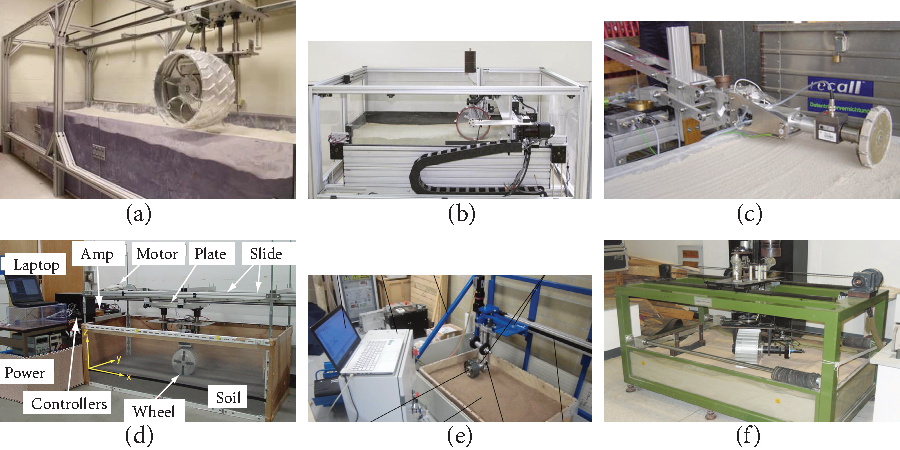
\includegraphics[width=6.5in]{general-images/existing-test-rigs.pdf}
\caption{Existing single-wheel test rigs at various academic and research institutions. (a) MIT Single Wheel Test Rig \cite{senatore2014modeling}; (b) CMU Single Wheel Soil Imaging Testbed \cite{moreland2012soil}; (c) ESA ExoMars Project Single Wheel Test Rig \cite{gallina2014parameter}; (d) Tohuku University Single Wheel Test Bed \cite{ishigami2008terramechanics}; (e) Politecnico di Torino Single Wheel Test Rig \cite{genta2016testing}; (f) Harbin Institute of Technology (HIT) Wheel-Soil Interaction Test Bed \cite{ding2013experimental}}
\label{fig:existing-test-rigs}
\end{figure}

\begin{table}[htpb!]
\caption{Summary of key characteristics and capabilities of the various single wheel test rigs}
\label{tab:existing-test-rigs}
\begin{threeparttable}
\begin{tabular}{|c|c|c|c|c|c|c|}
  \hline
% after \\: \hline or \cline{col1-col2} \cline{col3-col4} ...
   & Length, & Linear & Tire &  Slip ratio & Slip angle & Camber angle \\
   & m &speed, mm/s & diameter, cm &  control & control & control \\
  \hline\hline
  MIT & 3.5 & 60 & 50 & Yes & No & No \\ \hline
  CMU  & 1.0\tnote{{a}} & 1.0 & 50 & Yes & No & No\\ \hline
  ESA RCET & 3.0\tnote{{a}} & n/a\tnote{{b}} & 25 & Yes & n/a\tnote{{b}} & n/a\tnote{{b}}\\ \hline
  Tohuku University & 2.0 & 35 & 20 & Yes & Yes & No\\ \hline
  Politecnico di Torino  & 2.7 & n/a\tnote{{b}} & 18 & Yes & Yes & Yes \\\hline
  HIT  & 1.7 & n/a\tnote{{b}} & 40 & Yes & Yes & No \\\hline
  Purdue OW Test Rig\tnote{{c}}  & 4.8 & 200 & 200 & Yes & Yes & Yes\\\hline
\end{tabular}
\begin{tablenotes}
\item[{a}] Estimated by the authors\\
\item[{b}] Data not available\\
\item[{c}] Proposed in this work
\end{tablenotes}
\end{threeparttable}
\end{table}


\section{Design and Fabrication of the Single Wheel Test Rig}
\label{sec:design-and-fabrication-of-test-rig}

The high-level objective(s) of the work described in this paper are as follows: 1) Design and construction of a single wheel test rig for Ocean World rovers, and 2) Construction of a prototype novel large-diameter deployable rover wheel. 3) Demonstrate the test rig capabilities using the prototype wheel under a range of slip ratios and other test conditions expected on Ocean World surfaces.  A detailed description of the design, fabrication, and design rationale of the prototype wheel is given in Section \ref{sec:tire-prototyoe-fabrication}. The requirements for the test rig are derived from these high-level objectives, and are described in the following subsections.

\subsection{System Requirements and Constraints}

The rig design is largely driven by the requirement to accommodate the prototype test tire which is approximately 1 meter in diameter and 25 cm in width.  During the early stage of the design, the team considered the choice between using a horizontally moving surface with the wheel held in place, as opposed to a static surface on which the wheel will be rolled over. While a moving underlying surface is ideally suited for flat surfaces and is widely used in the automobile industry for dynamic wheel testing, it presents inherent difficulties when more flexibility is required in terms of the nature of the surface.  To accommodate a wide range of surface features such as granular ice and boulder fields, the team decided to use a horizontally moving wheel over a static test bed which can be reconfigured with different surface conditions. 

The length of the test-rig is driven by empirical rule that the test should run for at least one wheel revolution to accommodate startup transients before the wheel reaches the desired slip conditions.  This imposed a requirement of at least 3.5 meters of usable test bed length. The maximum allowable footprint (due to space constraints) of the test rig footprint was 6.0 meters. Considering these constraints, the test rig is 6 m x 2 m x 2 m (length x width x height), and provides 4.5 meters of usable test bed length. 

The next major requirement is to be able to test the prototype wheel under a range of slip ratios. The wheel slip ratio $s$ is a non-dimensional parameter defined as follows \cite{ishigami2008terramechanics}.

\begin{equation}
        s =
        \left\{ \begin{array}{ll}
            (r\omega - v_x)/r\omega &  \text{if $|r\omega| > v_x$, positive slip} \\
             (r\omega - v_x)/v_x &  \text{if $|r\omega| < v_x$, negative slip} 
        \end{array} \right.
    \end{equation}

where $r$ is the wheel radius, $\omega$ is the wheel angular speed, and $v_x$ is the wheel horizontal speed. A desired slip ratio is achieved by providing independent control of both the wheel angular speed and the wheel horizontal speed. Planetary rovers typically operate at very low speeds ($<$ 0.1 m/s), and hence most existing single wheel test rigs are designed to operate at such speeds as seen in Table \ref{tab:existing-test-rigs}. Figure \ref{fig:slip-ratio-chart} shows the required wheel angular speed as a function of the wheel horizontal speed for a range of slip ratios. Ideally, the test rig should be capable of accommodating the entire theoretical range of slip ratios for any given horizontal speed. However, as seen in Figure \ref{fig:slip-ratio-chart}, this is not realizable as the required angular velocity increases sharply as the slip ratio approaches 1.0. The selected operating range for $\omega$ and $v_x$ are shown in green in Fig. \ref{fig:slip-ratio-chart} which allows slip ratios as high as 0.8 for a nominal horizontal speed of 0.1 m/s. The upper limit for $v_x$ of 0.2 m/s is an arbitrary design requirement based on expected the expected speed of a future planetary rover, and to achieve negative slip values with reasonably large $\omega$ ($> 0.2$ rad/s) as shown in Fig. \ref{fig:slip-ratio-chart}. 


\begin{figure}[hbt!]
\centering
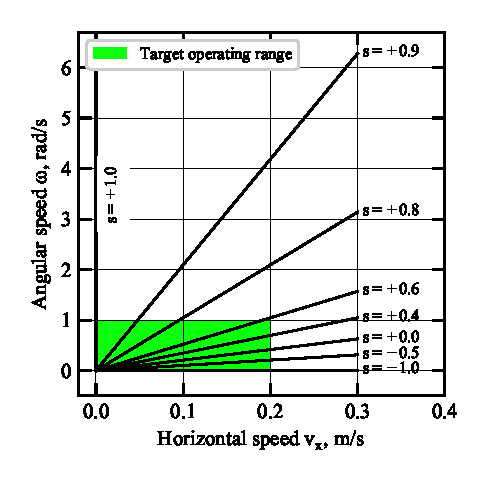
\includegraphics[width=3.15in]{plots/slip-ratios.eps}
\caption{Required wheel angular speed as a function of horizontal travel speed at various slip ratios (for the prototype test wheel with diameter = 0.956 m)}
\label{fig:slip-ratio-chart}
\end{figure}

The vertical load on the wheel $F_v$ is another important test parameter, and must be controlled to simulate the wheel-soil interaction on planetary surfaces with different values of surface gravity. The prototype test wheel is intended to be used on a 4-wheel rover weighing approximately 800 kg which will be delivered to Europa's surface using an MSL-derived skycrane descent system. Taking into account Europa's surface gravity of 1.32 m/s\textsuperscript{2}, this results in a vertical load of 264 N. The corresponding loads on Mars, Titan and Enceladus are 270 N and 22 N respectively. If the vehicle is moving up or down a slope, the local vertical component of the force will be smaller as defined by the slope angle.  Considering these loads, the requirement for the vertical load on the wheel is in the range of 20--400 N. The nominal  load accuracy requirement is arbitrarily set to 1\% of the desired value, though this may not be practical at very low vertical loads. 

The requirements for slip angle $\alpha$ and camber angle $\beta$ (as illustrated in Fig. \ref{fig:slip-camber-schmatic}) are both arbitrarily defined as $\pm$25 degrees, which is a nominal upper bound for the range of these angles expected for planetary rovers. The test bed is to be able to accommodate the prototype 25 cm wide wheel in the slip and camber angle geometries, and is required to be at least 70 cm wide and 30 cm deep. The test bed is required to be able to be simulate a wide range of conditions which may be expected on icy moons such as Europa. Figure \ref{fig:icy-moon-photos-and-earth-analogs} shows some of the highest resolution photographs of Europa and Enceladus from the Galileo and Cassini-Huygens spacecraft. As a starting point the test bed is required to able to accommodate granular ice simulant, boulder fields, sharp ice formations and also provide a flat hard surface resembling smooth ice. Laboratory studies using both observational data from spacecraft and telescopes, experimental studies of water ice under cryogenic and  vacuum conditions are currently underway. Analog sites such as the ones shown in Fig. \ref{fig:earth-analog-sites} may offer some insight into the conditions on these icy worlds, though ice is known to behave very differently under cryogenic conditions than that encountered on Earth.  As more data becomes available, other test bed simulants and surface features may be used to provide more realistic representation of the icy moon surfaces. 

\begin{figure}[hbt!]
\centering
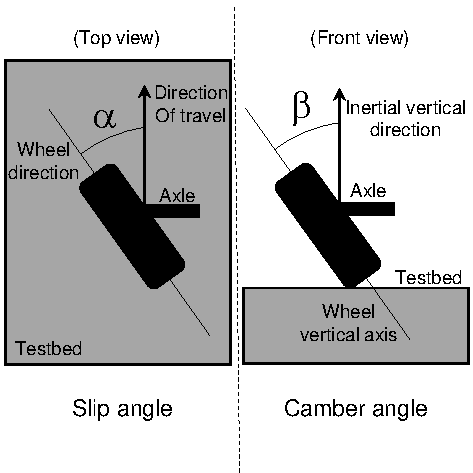
\includegraphics[width=3.00in]{general-images/slip-camber-schematic.pdf}
\caption{Schematic illustrating slip and camber angles.}
\label{fig:slip-camber-schmatic}
\end{figure}

\begin{figure}[hbt!]
\centering
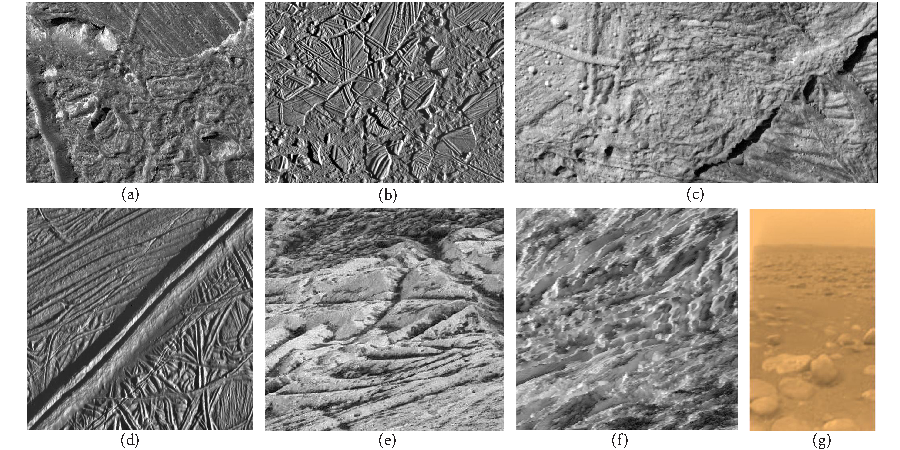
\includegraphics[width=6.5in]{general-images/icy-moon-surfaces.pdf}
\caption{High resolution images showing the varied surface features on Ocean Worlds. (a) Very high resolution view of the Conamara Chaos on Europa. The image is 5 km wide and shows a rugged surface with ice blocks that have been broken up and then frozen. Credit: NASA/JPL/PIA01177. (b) High resolution image of Europa's jumbled crustal plates, showing an area 42 km wide. Credit: NASA/JPL/PIA00591. (c) High resolution image of Europa' surface showing numerous impact craters amid rugged terrain, image is 8 km wide. Credit: NASA/JPL/PIA01404. (d) Close-up image of one of Europa's ubiquitous double ridges. The ridge is 2.6 km wide and rises to about 300 m. Credit: NASA/JPL/PIA00589. (e) Highest resolution image of Europa showing an area 1.8 km wide. Credit: NASA/JPL/PIA01180. (f) Close-up view of Enceladus, showing an area 7.6 km wide. Credit: NASA/JPL/PIA17204. (g) Titan's surface as seen by the Huygens probe showing pebble-sized ice blocks about 15 cm across. Credit: NASA/JPL/ESA/PIA07232.}
\label{fig:icy-moon-photos-and-earth-analogs}
\end{figure}

\begin{figure}[hbt!]
\centering
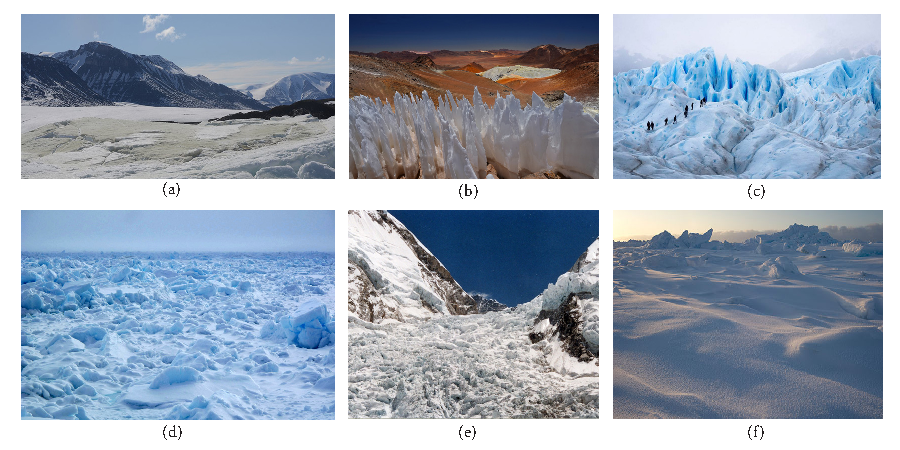
\includegraphics[width=6.5in]{general-images/earth-analog-sites.pdf}
\caption{Various ice formations on Earth, some of which may be representative of the landscapes on icy moons such as Europa and Enceladus. (a) Sulfidic outcrop (yellow colored marking on the ice) in Borup Fiord Pass glacier, Ellesmere Island in the Canadian High Arctic. A sulfur-rich spring passes under glacial ice before emerging onto the surface, making it one of the most interesting Earth-analog sites for Europa from an astrobiological perspective. Whether it presents an analog for the terrain is currently not known, but relatively smooth and flat terrain is likely present at some locations on Europa, and will be attractive landing sites from a safety perspective. Credit: NASA Astrobiology Website, John Spear at the Colorado School of Mines. (b) Penitents on the Cerro Toco volcano in the Atacama Desert in Chile. Such sharp ice features formed in dry high altitude are formed by differential ablation and are known to reach several meters in height. Penitents have been discovered on Pluto \cite{moores2017penitentes}, and may be present at Europa at some latitudes \cite{hobley2018formation}. Credit: Federico Ce, www.trekearth.com. (c) Extremely rugged ice formations in the Perito Moreno Glacier in Argentina, note the people for scale. Such terrain is likely present on icy moons and presents formidable challenges for mobility systems, though non-conventional systems such as snake-like robots may be more suited than wheeled rovers. Credit: www.macdermottsargentina.com. (d) Sea ice floating off the coast north of Barrow, Alaska. Credit: Ned Rozell/University of Alaska, Fairbanks. (e) Jumbled up ice blocks each several tens of meters to a few meters in size at the Khumbu Icefall in Nepal en-route to Mt. Everest. Sites such as the Conamara Chaos on Europa which shows activity of relatively recent (in geologic timescales) interaction with the underlying liquid water ocean will likely feature such extremely rugged terrain. Credit: Uwe Gille, Wikipedia, CC-BY-SA-3.0. (f) Powdery snow on sea ice near Barrow, Alaska. Credit: Chris Linder/University of Washington. Such terrain is likely present at Enceladus' south polar regions from freshly fallen material ejected from the active geysers \cite{porco2006cassini}, and may present a hazard for landers and rovers which may sink into the surface.}
\label{fig:earth-analog-sites}
\end{figure}

The most important measurements of interest are the forces and moments on the wheel as it rolls across the surface under different test conditions, and is accomplished using 6-axis Force Torque (FT) sensor. Figure \ref{fig:wheel-forces-and-moments} shows the wheel coordinate system centered at the wheel hub and the definition of the drawbar pull $F_X$, lateral force $F_Y$, normal force $F_Z$, lateral rolling moment $M_X$, drive torque $M_Y$, and the aligning torque $M_Z$. \textcolor{teal}{@Ye: mention the measurement requirements for the FT sensor here.} Wheel displacement in the vertical direction is required to measure sinkage, and along the horizontal direction to measure wheel slippage. 

\begin{figure}[hbt!]
\centering
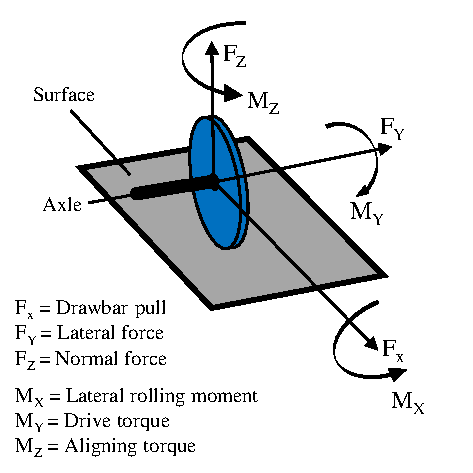
\includegraphics[width=3.15in]{general-images/wheel-forces-and-moments.pdf}
\caption{Wheel forces and moments.}
\label{fig:wheel-forces-and-moments}
\end{figure}


\subsection{Mechanical System Design}


\subsubsection{Superstructure}


\subsubsection{Carriage Motion}
\label{subsubsec:carriage-motion}

\subsection{Electrical System Design}

\section{Tire Prototype Fabrication}
\label{sec:tire-prototyoe-fabrication}


\section{Experimental Setup and Procedure}


\section{Verification and Validation}


\section{Sample Test Results with Prototype Tire}

\section{Conclusions}

This is the conclusion.

\subsubsection*{Acknowledgments}
This is the acknowledgement.

\bibliographystyle{apalike}
\bibliography{references}

\end{document}